\section{\MakeUppercase{Results and Analysis}}
This section covers the results and analysis of the models, including loss curves, audio analysis, comparisons with traditional codecs, and the effects of quantization.

\subsection{Teacher Model Loss Curves}

\begin{figure}[H]
    \centering
    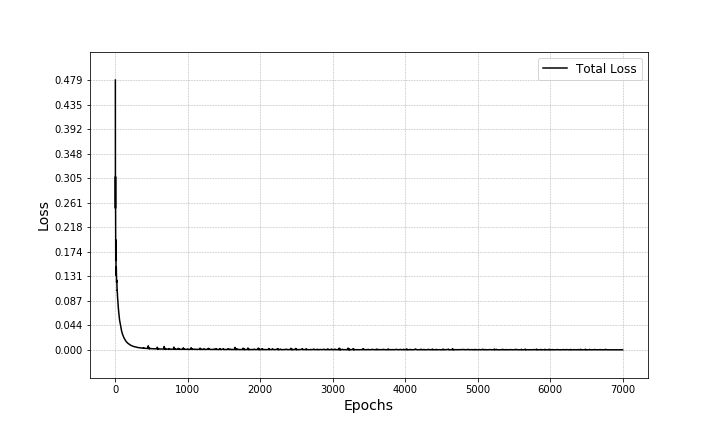
\includegraphics[height=0.6\linewidth]{assets/audio_video_loss_curves/video1_loss.png}
    \caption{Teacher Model Training Loss Curve for Video 1}
    \label{fig:video-loss-curve-1}
\end{figure}

\begin{figure}[H]
    \centering
    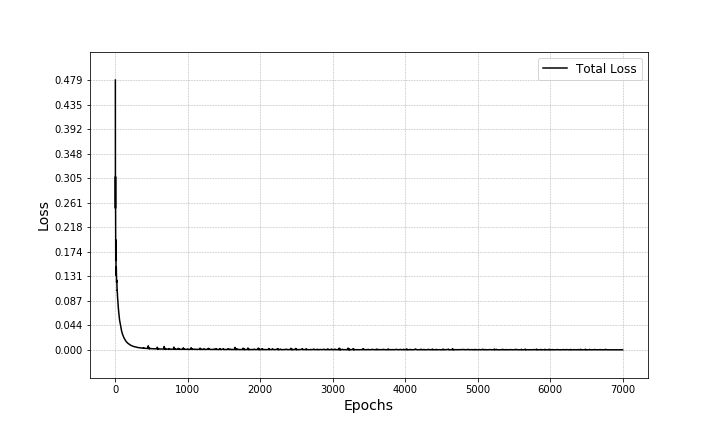
\includegraphics[height=0.6\linewidth]{assets/audio_video_loss_curves/video1_loss.png}
    \caption{Teacher Model Training Loss Curve for Video 2}
    \label{fig:video-loss-curve-2}
\end{figure}

\begin{figure}[H]
    \centering
    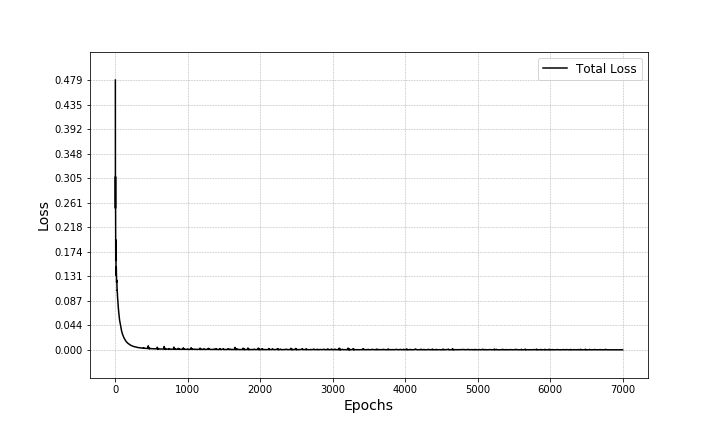
\includegraphics[height=0.6\linewidth]{assets/audio_video_loss_curves/video1_loss.png}
    \caption{Teacher Model Training Loss Curve for Video 3}
    \label{fig:video-loss-curve-3}
\end{figure}

\begin{figure}[H]
    \centering
    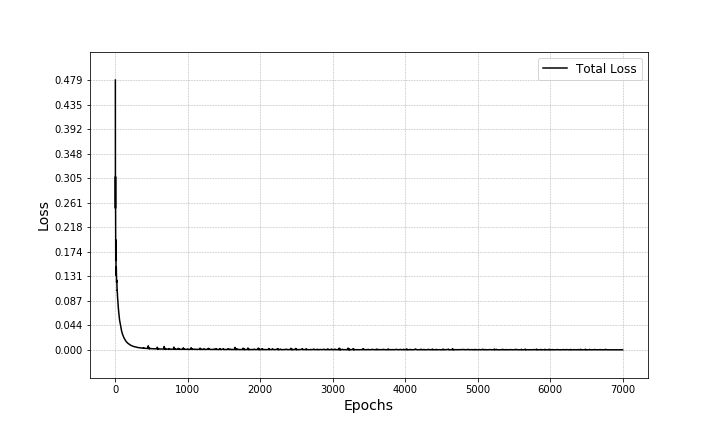
\includegraphics[height=0.6\linewidth]{assets/audio_video_loss_curves/video1_loss.png}
    \caption{Teacher Model Training Loss Curve for Video 4}
    \label{fig:video-loss-curve-4}
\end{figure}

\begin{figure}[H]
    \centering
    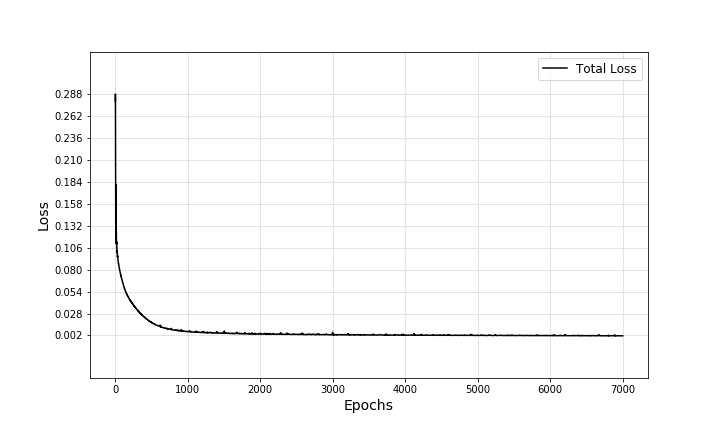
\includegraphics[height=0.6\linewidth]{assets/audio_video_loss_curves/video5_loss.png}
    \caption{Teacher Model Training Loss Curve for Video 5}
    \label{fig:video-loss-curve-5}
\end{figure}


The loss values for the model start at a low level and show a very steep decline, approaching nearly zero around epoch 500. After this point, the rate of decline in the loss slows down almost being linear. Although the loss value approaches zero, training continues beyond this point. This is because even though there were only minute improvements in the loss function the performance metrics such as \gls{psnr}, \gls{ssim}, \gls{lpips}, \gls{lsd} were improving. The continued training ensured that these evaluation metrics were optimized, further enhancing the quality of the video representation model.

\subsection{Student Model Loss Curves}

\begin{figure}[H]
    \centering
    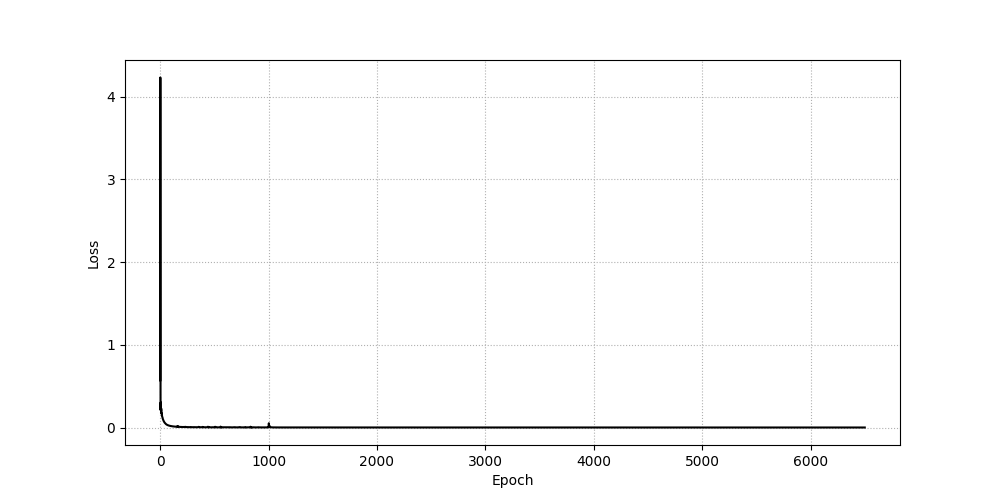
\includegraphics[width=1\linewidth,height=0.6\linewidth]{assets/quantization/student_vvsa_loss_curve.png}
    \caption{Student Model Training Loss Curve of Video 1}
    \label{fig:student-video-loss-curve-1}
\end{figure}

\begin{figure}[H]
    \centering
    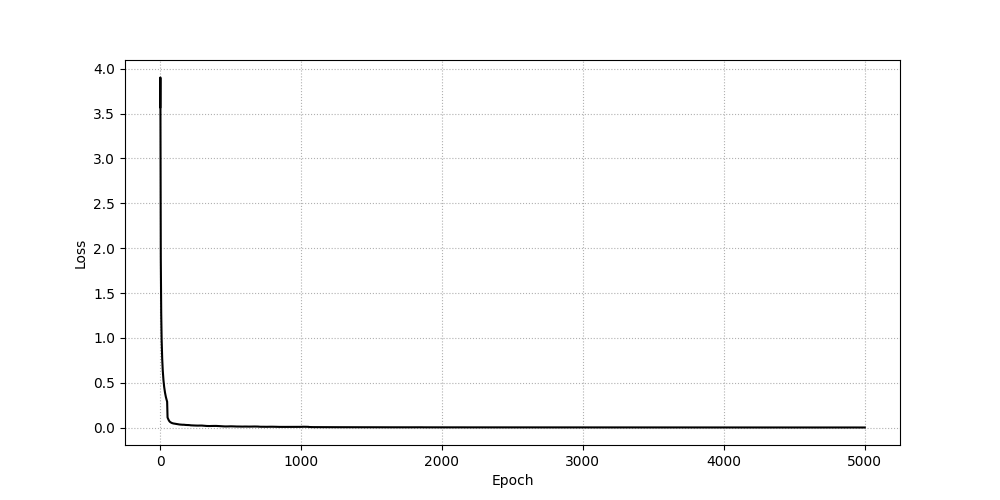
\includegraphics[width=1\linewidth,height=0.6\linewidth]{assets/quantization/student_rick_loss_curve.png}
    \caption{Student Model Training Loss Curve of Video 3}
    \label{fig:student-video-loss-curve-3}
\end{figure}

Initially, the loss begins at a relatively high value, with a sharp and rapid decline within the first few hundred epochs, indicating significant progress in optimizing the model. Within epoch 200, the loss value stabilizes and approaches nearly zero, with further reductions becoming progressively smaller and almost linear in trend. Although the improvements in the loss function become minimal after this point, training continues in the same manner as for the teacher models.

\subsection{FFT and Spectrogram Analysis of Audio Content Across Videos}
This section provides a visual analysis of the fidelity of the audio predictions by comparing the ground truth and predicted signals in both the time and frequency domains.

\begin{figure}[H]
    \centering
    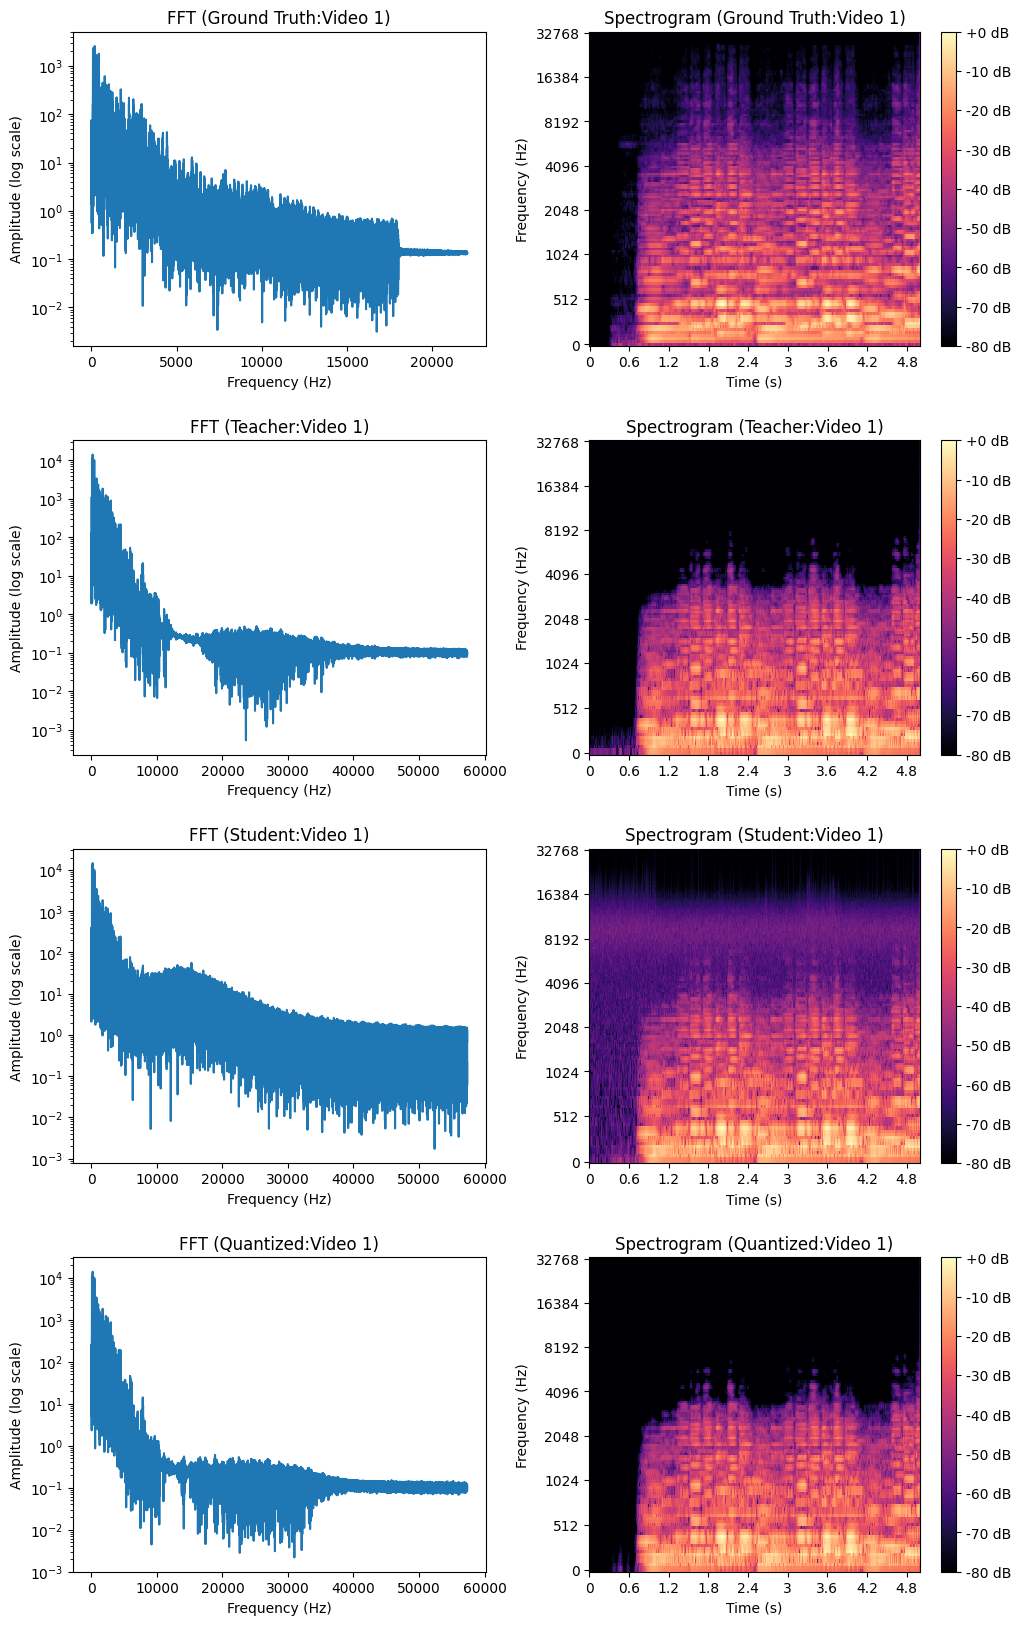
\includegraphics[width=0.8\linewidth]{assets/quantization/fft_spectrogram_Video1.png}
    \caption{FFT and Spectrogram Analysis of Audio Content in Video 1}
    \label{fig:fft-spec-v1}
\end{figure}

\begin{figure}[H]
    \centering
    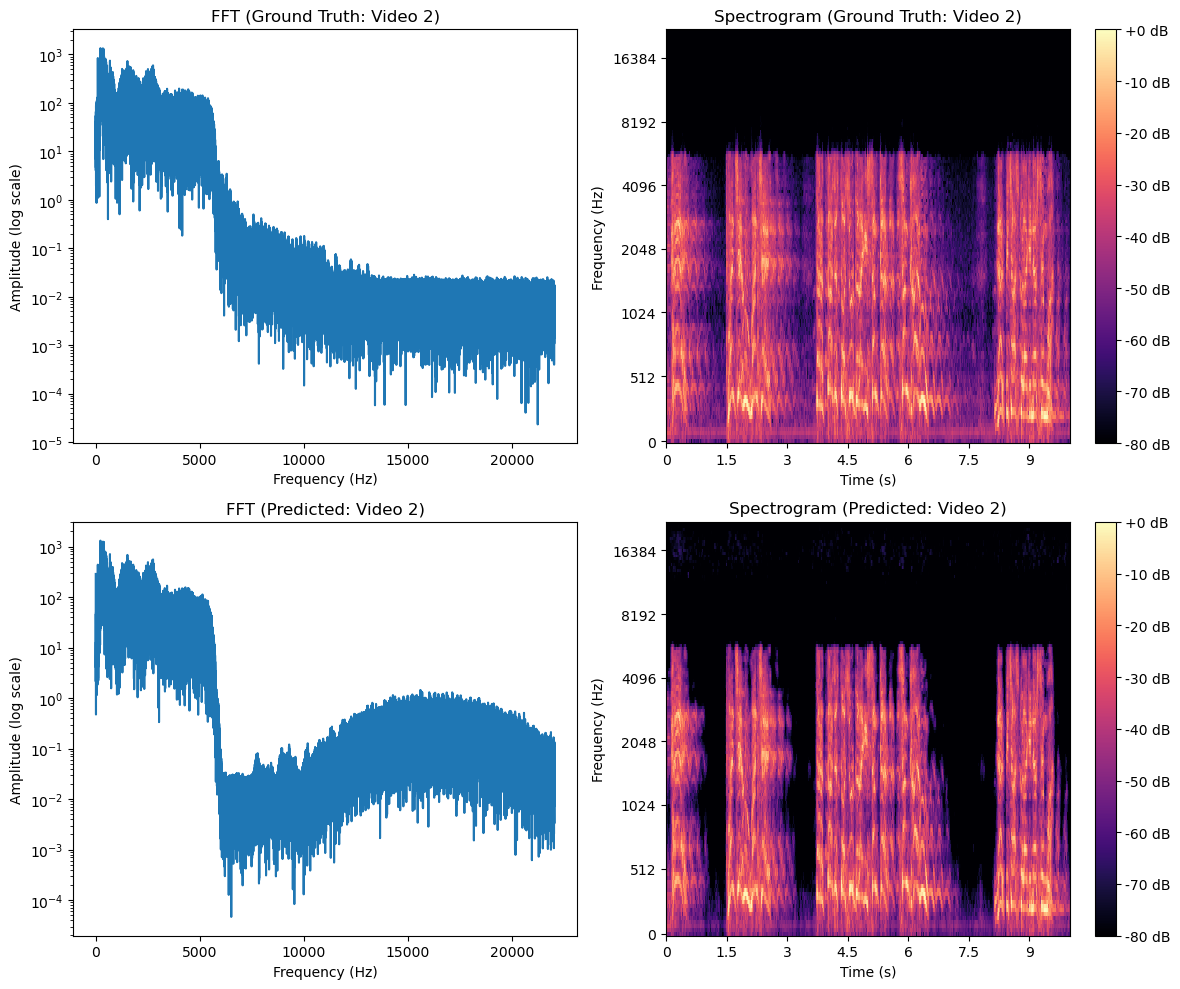
\includegraphics[width=0.8\linewidth]{assets/audio_video_analysis/Video_2_analysis.png}
    \caption{FFT and Spectrogram Analysis of Audio Content in Video 2}
    \label{fig:fft-spec-v2}
\end{figure}

\begin{figure}[H]
    \centering
    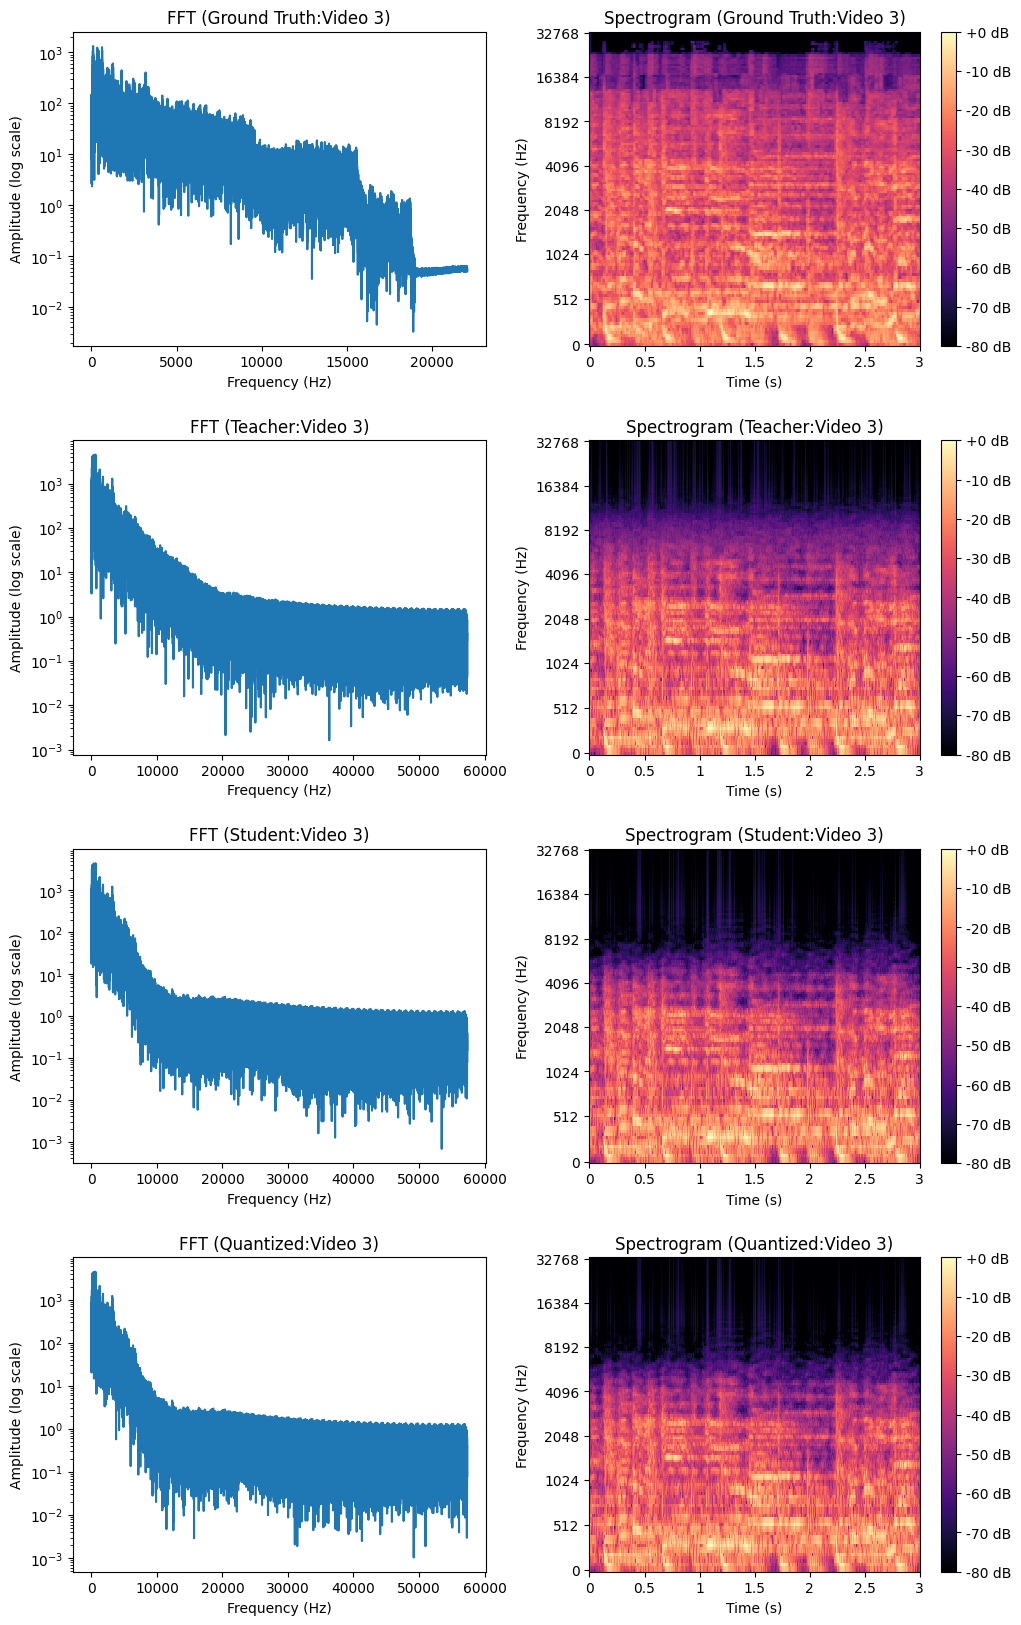
\includegraphics[width=0.7\linewidth]{assets/quantization/fft_spectrogram_Video3.png}
    \caption{FFT and Spectrogram Analysis of Audio Content in Video 3}
    \label{fig:fft-spec-v3}
\end{figure}

\begin{figure}[H]
    \centering
    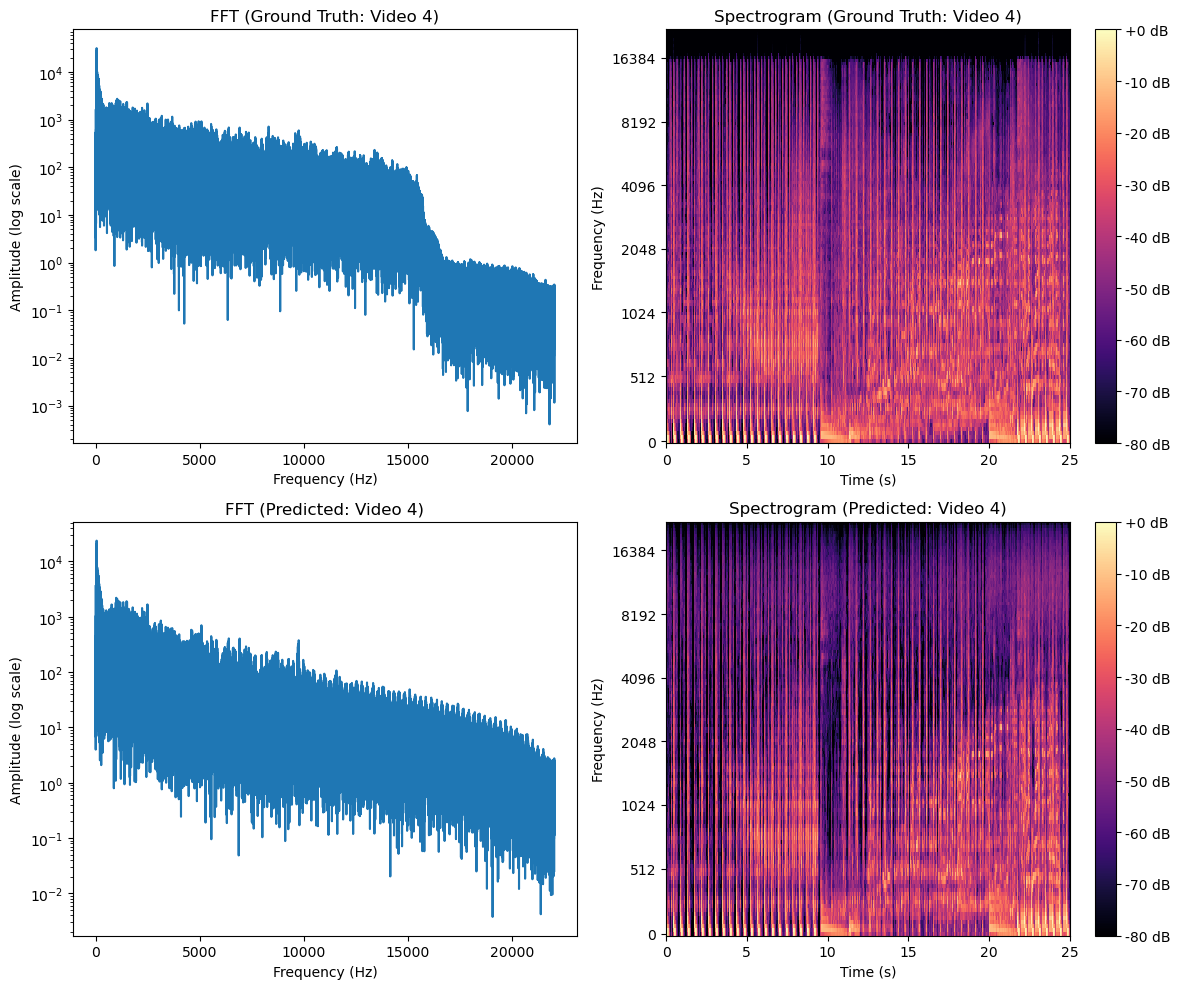
\includegraphics[width=0.8\linewidth]{assets/audio_video_analysis/Video_4_analysis.png}
    \caption{FFT and Spectrogram Analysis of Audio Content in Video 4}
    \label{fig:fft-spec-v4}
\end{figure}

\begin{figure}[H]
    \centering
    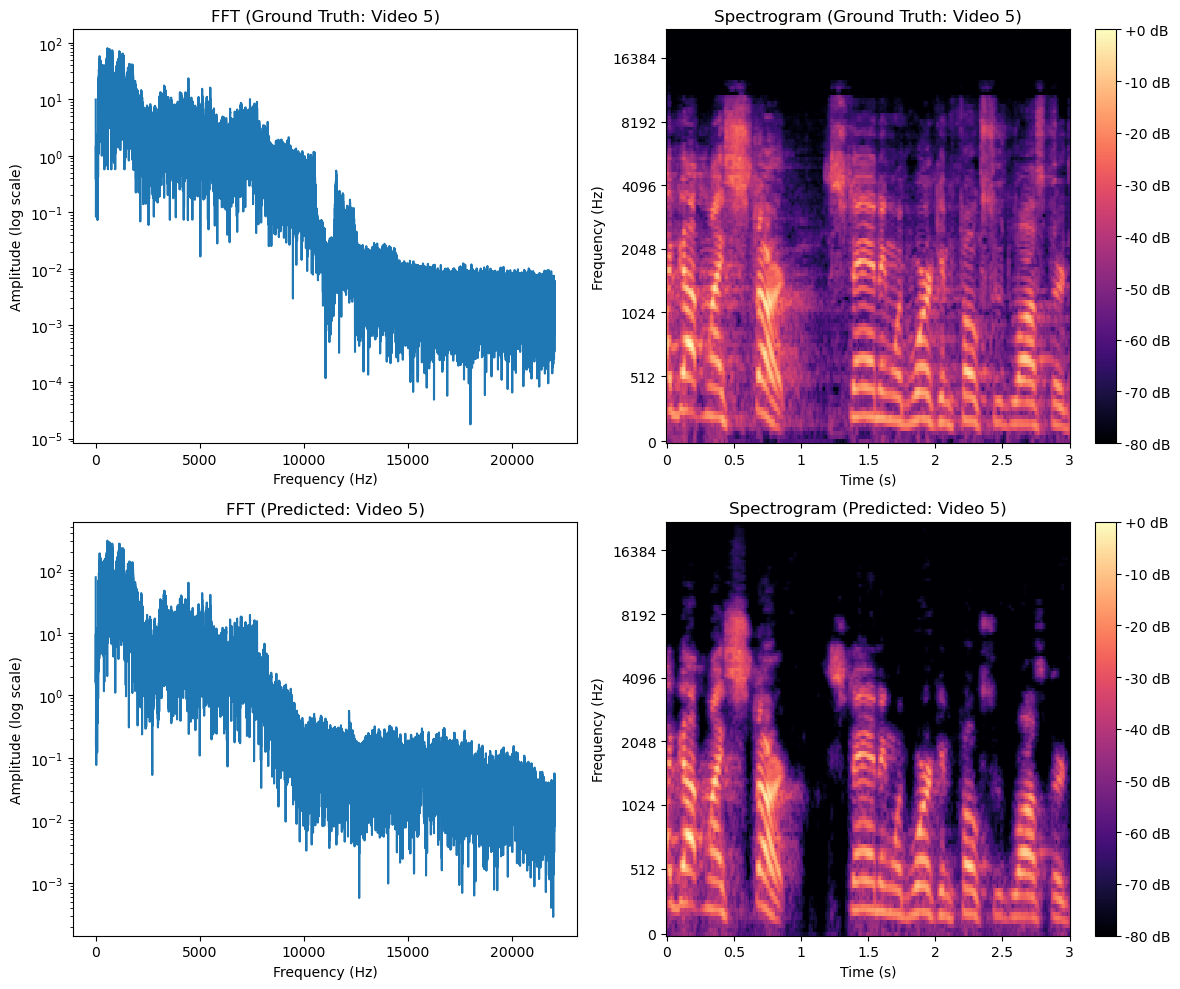
\includegraphics[width=0.8\linewidth]{assets/audio_video_analysis/Video_5_analysis.png}
    \caption{FFT and Spectrogram Analysis of Audio Content in Video 5}
    \label{fig:fft-spec-v5}
\end{figure}

The \gls{fft} and spectrogram plots of the audio content in the inferenced videos closely resemble the ground truth plots across all videos. The model successfully recreates the audio signals with various frequency components, although slight deviations are observed in the FFT plots. However, the spectrograms remain almost identical across all videos, demonstrating the model's ability to capture the temporal structure of the audio. 

In the spectrogram of Video 2 and Video 5, a slight loss of signal is noticable, which can be attributed to the application of the noise reduction algorithm. This algorithm appears to have mistakenly identified some parts of the signal as noise and removed them, leading to this minor discrepancy.


\subsection{Comparision with Traditional Codecs}
    \subsubsection{Performance Metrics of Teacher Model}
    \begin{table}[H]
        \centering
        \caption{Video Metrics of Teacher Model}
        \label{table:video-metric-teacher}
        \begin{tabular}{|c|c|c|c|c|c|c|}
        \hline
        \multirow{2}{*}{\textbf{Video}} & \textbf{PSNR} & \multirow{2}{*}{\textbf{LPIPS}} & \multirow{2}{*}{\textbf{SSIM}} & \textbf{Original} & \textbf{Model Size} & \textbf{Compression} \\
        & \textbf{(dB)} &  &  & \textbf{Size (KiB)} & \textbf{(KiB)} & \textbf{Ratio} \\
        \hline
        Video 1 & 42.69 & 0.05 & 0.98 & 1972 & \multirow{5}{*}{9260} & 0.21 \\
        \cline{1-5} \cline{7-7}
        Video 2 & 35.08 & 0.17 & 0.92 & 5462 &  & 0.58 \\
        \cline{1-5} \cline{7-6}
        Video 3 & 21.88 & 0.39 & 0.67 & 6235 &  & 0.67 \\
        \cline{1-5} \cline{7-7}
        Video 4 & 26.89 & 0.41 & 0.72 & 14018 &  & 1.50 \\
        \cline{1-5} \cline{7-7}
        Video 5 & 32.88 & 0.21 & 0.92 & 12781 &  & 1.37 \\
        \hline
        \end{tabular}
    \end{table}
    
    \begin{table}[H]
        \centering
        \caption{Audio Metrics of Teacher Model}
        \label{table:audio-metric-teacher}
        \begin{tabular}{|c|c|c|c|}
        \hline
        \multirow{2}{*}{\textbf{Video}} & \textbf{PSNR} & \textbf{LSD} & \multirow{2}{*}{\textbf{ViSQOL}}\\
        & \textbf{(dB)} & \textbf{(dB)} &  \\
        \hline
        Video 1 & 57.57 & 4.50 & 3.54 \\
        \hline
        Video 2 & 57.09 & 4.28 & 3.35 \\
        \hline
        Video 3 & 62.50 & 7.60 & 4.51 \\
        \hline
        Video 4 & 64.33 & 8.15 & 3.58 \\
        \hline
        Video 5 & 46.60 & 6.89 & 2.66 \\
        \hline
        \end{tabular}
    \end{table}

    \autoref{table:video-metric-teacher} presents the video metrics of the teacher model, showing the \gls{psnr}, \gls{lpips}, \gls{ssim}, original video size, model size, and compression ratio for five different videos. The \gls{psnr} values range from 21.88 dB to 42.69 dB, indicating a notable variation in video quality. Video 1 achieves the highest \gls{psnr} at 42.69 dB, demonstrating superior quality compared to the other videos. In contrast, Video 3 has the lowest \gls{psnr} of 21.88 dB, reflecting a lower-quality reconstruction. The \gls{ssim} values remain high, suggesting that the model preserves structural details well across all videos, with values ranging from 0.67 to 0.98. The compression ratios vary from 0.21 for Video 1 to 1.50 for Video 4, showing how compression affects the model's storage efficiency and output size.

    \autoref{table:audio-metric-teacher} shows the audio metrics for the teacher model, including \gls{psnr}, \gls{lsd}, and \gls{visqol} scores for each video. The \gls{psnr} values indicate high fidelity, with Video 3 achieving the highest \gls{psnr} at 62.50 dB, while Video 5 has the lowest at 46.60 dB. The \gls{lsd} values indicate the level of distortion, with Video 1 having the lowest value of 4.50 dB, signifying better quality. The \gls{visqol} scores, which evaluate perceptual quality, show consistency across most videos, with Video 3 achieving the highest score of 4.51. Overall, the audio metrics indicate that the teacher model performs well, but there is a slight decline in performance for Video 5, particularly in terms of \gls{psnr} and \gls{visqol}.


\subsubsection{Performance Metrics of Student Model with Quantization}
    Quantization impacts the quality of reconstructed images and audio, as measured by PSNR, SSIM and LSD. It also reduces file size. The following table shows the performance metrics for student model before and after quantization to 16-bit.

    \begin{table}[H]
        \centering
        \caption{Metrics Before and After Quantization of Student Model for Video 1}
        \label{tab:metrics-quantization-video-1}
        \begin{tabular}{|c|c|c|c|}
            \hline
            \multirow{2}{*}{\textbf{Metrics}} & \multicolumn{2}{c|}{\textbf{Value}} \\ \cline{2-3}
            & \textbf{Student Model} & \textbf{16-bit Quantization} \\ \hline
            \textbf{PSNR(Frames)(dB)} & 35.5525 & 35.3520 \\ \hline
            \textbf{SSIM} & 0.9194 & 0.9189 \\ \hline
            \textbf{LPIPS} & 0.0794 & 0.0848\\ \hline
            \textbf{PSNR(Audio)(dB)} & 18.7929 & 18.8487  \\ \hline
            \textbf{LSD(dB)} & 4.5930 & 4.8484 \\ \hline
            % \textbf{VISQOL} & & \\ \hline
            \textbf{SQNR(dB)} & - & 39.214 \gls{db} \\ \hline
            \textbf{File Size(MiB)} & 4.96 & 2.48 \\ \hline
            \textbf{Compression Ratio} & 0.38 & 0.77 \\ \hline
        \end{tabular}
    \end{table}

    The results from the \autoref{tab:metrics-quantization-video-1} demonstrate the effect of quantization on both video and audio quality for Video 1. A significant reduction in file size is observed, dropping from 4.96 \gls{mib} to 2.48 \gls{mib}, a 50\% reduction. Despite this compression, the quality metrics indicate only minor degradation. The PSNR for the video frames decreased slightly from 35.5525 \gls{db} to 35.3520 \gls{db}, showing that the overall visual quality remains almost unchanged post-quantization. Similarly, the \gls{ssim} metric, which measures structural similarity, experienced a marginal decrease from 0.9194 to 0.9189, indicating that the structural integrity of the video is nearly preserved.

    The \gls{sqnr} value at 39.214 \gls{db} provides a robust measure of the quantization noise introduced during the compression process. This relatively high value suggests that the noise is effectively controlled, ensuring that the perceived quality remains satisfactory. The audio metrics show a slight improvement, with the \gls{psnr} increasing from 18.7929 \gls{db} to 18.8487 \gls{db}, suggesting that the audio quality benefits slightly from the quantization process. However, the \gls{lsd} value increased from 4.5930 \gls{db} to 4.8484 \gls{db}, indicating a slight degradation in the audio frequency spectrum. Nevertheless, this change is minimal and does not significantly affect the overall audio experience. The overall file size reduction highlights the efficiency of quantization in compressing both video and audio, with manageable trade-offs in quality.

    \begin{table}[H]
        \centering
        \caption{Metrics Before and After Quantization of Student Model for Video 3}
        \label{tab:metrics-quantization-video-3}
        \begin{tabular}{|c|c|c|c|}
            \hline
            \multirow{2}{*}{\textbf{Metrics}} & \multicolumn{2}{c|}{\textbf{Value}} \\ \cline{2-3}
            & \textbf{Student Model} & \textbf{16-bit Quantization} \\ \hline
            \textbf{PSNR(Frames)(dB)} & 28.8588 & 28.7153 \\ \hline
            \textbf{SSIM} & 0.7579 & 0.7529 \\ \hline
            \textbf{LPIPS} & 0.4039 & 0.4126 \\ \hline
            \textbf{PSNR(Audio)(dB)} & 24.1992 & 24.1786 \\ \hline
            \textbf{LSD(dB)} & 10.7038 & 10.6928 \\ \hline
            \textbf{File Size(MiB)} & 4.96 & 2.48 \\ \hline
            \textbf{Compression Ratio} & 1.22 & 2.45\\ \hline
        \end{tabular}
    \end{table}

    The results in \autoref{tab:metrics-quantization-video-3} show the impact of quantization on Video 2. As with Video 1, the file size is reduced by 50\%, from 4.96 \gls{mib} to 2.48 \gls{mib}, demonstrating the effectiveness of quantization in compressing the video. The \gls{psnr} for video frames decreased slightly from 28.8588 \gls{db} to 28.7153 \gls{db}, indicating minimal visual quality degradation, and the \gls{ssim} dropped marginally from 0.7579 to 0.7529, suggesting that the structural integrity is similarly well-preserved.

    For the audio, the \gls{psnr} showed a negligible change, from 24.1992 \gls{db} to 24.1786 \gls{db}, and the \gls{lsd} remained almost the same, moving from 10.7038 \gls{db} to 10.6928 \gls{db}, further confirming that the audio quality remains stable after quantization. Overall, the results are consistent with those observed in Video 1, indicating a good balance between file size reduction and quality retention.


    \subsubsection{Performance Metrics of Traditional Codecs}

    % Video Metrics Table
    \begin{table}[H]
        \centering
        \caption{Metrics for Video Content of Video 1}
        \label{table:vid-met-1}
        \begin{tabular}{|c|c|c|c|c|c|c|c|}
        \hline
        \multicolumn{8}{|c|}{\textbf{Video 1 (1972 KiB)}} \\ \hline
        \multirow{2}{*}{\textbf{Codec}} & \multirow{2}{*}{\textbf{CRF}} & \textbf{Bitrate} & \textbf{PSNR} & \textbf{SSIM} & \textbf{LPIPS} & \textbf{File Size} & \textbf{Compression} \\ 
        &  & \textbf{(kbps)} & \textbf{(dB)} &  &  & \textbf{(KiB)} & \textbf{Ratio} \\ \hline
        \multirow{3}{*}{H.264/MP3} & 1  & 320 & 61.60 & 0.99 & 0.004 & 429.64  & 4.59 \\ \cline{2-8} 
                                & 23 & 192 & 47.24 & 0.99 & 0.005 & 178.59  & 11.04 \\ \cline{2-8} 
                                & 51 & 64  & 32.00 & 0.83 & 0.23 & 44.28   & 44.52 \\ \hline
        \multirow{3}{*}{H.265/MP3} & 1  & 320 & 59.53 & 0.99 & 0.004 & 378.32  & 5.21 \\ \cline{2-8} 
                                & 28 & 192 & 45.32 & 0.98 & 0.02 & 154.51  & 12.76 \\ \cline{2-8} 
                                & 51 & 64  & 33.37 & 0.85 & 0.21 & 45.70   & 43.14 \\ \hline
        \end{tabular}
    \end{table}

    \begin{table}[H]
        \centering
        \caption{Metrics for Audio content of Video 1}
        \label{table:aud-met-1}
        \begin{tabular}{|c|c|c|c|c|}
        \hline
        \textbf{Codec} & \textbf{Bitrate (kbps)} & \textbf{PSNR (dB)} & \textbf{LSD} & \textbf{VISQOL} \\ \hline
        \multirow{3}{*}{MP3} & 64  & 35.34 & 1.97 & 4.66 \\ \cline{2-5} 
                                   & 192 & 43.28 & 0.42 & 4.73 \\ \cline{2-5} 
                                   & 320 & 64.78 & 0.10 & 4.73 \\ \hline
        \end{tabular}
    \end{table}
    
    

    \begin{table}[H]
        \centering
        \caption{Metrics for Video Content of Video 2}
        \label{table:vid-met-2}
        \begin{tabular}{|c|c|c|c|c|c|c|c|}
        \hline
        \multicolumn{8}{|c|}{\textbf{Video 2 (5462 KiB)}} \\ \hline
        \multirow{2}{*}{\textbf{Codec}} & \multirow{2}{*}{\textbf{CRF}} & \textbf{Bitrate} & \textbf{PSNR} & \textbf{SSIM} & \textbf{LPIPS} & \textbf{File Size} & \textbf{Compression} \\ 
        &  & \textbf{(kbps)} & \textbf{(dB)} &  &  & \textbf{(KiB)} & \textbf{Ratio} \\ \hline
        \multirow{3}{*}{H.264/MP3} & 1  & 320 & 59.70 & 0.99 & 0.003 & 632 & 2.67 \\ \cline{2-8} 
                                & 23 & 192 & 44.94 & 0.98 & 0.005 & 190 & 8.87 \\ \cline{2-8} 
                                & 51 & 64  & 27.75 & 0.78 & 0.22 & 12  & 140.50 \\ \hline
        \multirow{3}{*}{H.265/MP3} & 1  & 320 & 52.13 & 0.99 & 0.004 & 434 & 3.88 \\ \cline{2-8} 
                                & 28 & 192 & 41.57 & 0.97 & 0.01 & 128 & 13.17 \\ \cline{2-8} 
                                & 51 & 64  & 27.83 & 0.76 & 0.29 & 14  & 120.40 \\ \hline
        \end{tabular}
    \end{table}
    

    \begin{table}[H]
        \centering
        \caption{Metrics for Audio content of Video 2}
        \label{table:aud-met-2}
        \begin{tabular}{|c|c|c|c|c|}
        \hline
        \textbf{Codec} & \textbf{Bitrate (kbps)} & \textbf{PSNR (dB)} & \textbf{LSD} & \textbf{VISQOL} \\ \hline
        \multirow{3}{*}{MP3} & 64  & 38.99 & 0.73 & 4.72 \\ \cline{2-5} 
                                   & 192 & 45.82 & 0.04 & 4.73 \\ \cline{2-5} 
                                   & 320 & 86.68 & 0.01 & 4.73 \\ \hline
        \end{tabular}
    \end{table}
    




    \begin{table}[H]
        \centering
        \caption{Metrics for Video Content of Video 3}
        \label{table:vid-met-3}
        \begin{tabular}{|c|c|c|c|c|c|c|c|}
        \hline
        \multicolumn{8}{|c|}{\textbf{Video 3 (6235 KiB)}} \\ \hline
        \multirow{2}{*}{\textbf{Codec}} & \multirow{2}{*}{\textbf{CRF}} & \textbf{Bitrate} & \textbf{PSNR} & \textbf{SSIM} & \textbf{LPIPS} & \textbf{File Size} & \textbf{Compression} \\ 
        &  & \textbf{(kbps)} & \textbf{(dB)} &  &  & \textbf{(KiB)} & \textbf{Ratio} \\ \hline
        \multirow{3}{*}{H.264/MP3} & 1  & 320 & 58.39 & 0.98 & 0.16 & 1218.82 & 5.12 \\ \cline{2-8} 
                                   & 23 & 192 & 42.22 & 0.96 & 0.16 & 161.85  & 38.52 \\ \cline{2-8} 
                                   & 51 & 64  & 22.17 & 0.72 & 0.34 & 31.65   & 196.98 \\ \hline
        \multirow{3}{*}{H.265/MP3} & 1  & 320 & 56.07 & 0.99 & 0.16 & 861.80  & 7.23 \\ \cline{2-8} 
                                   & 28 & 192 & 40.20 & 0.96 & 0.18 & 113.02  & 55.16 \\ \cline{2-8} 
                                   & 51 & 64  & 24.16 & 0.73 & 0.35 & 31.42   & 198.39 \\ \hline
        \end{tabular}
    \end{table}
    


    \begin{table}[H]
        \centering
        \caption{Metrics for Audio content of Video 3}
        \label{table:aud-met-3}
        \begin{tabular}{|c|c|c|c|c|}
        \hline
        \textbf{Codec} & \textbf{Bitrate (kbps)} & \textbf{PSNR (dB)} & \textbf{LSD} & \textbf{VISQOL} \\ \hline
        \multirow{3}{*}{MP3} & 64  & 27.99 & 4.21 & 4.64 \\ \cline{2-5} 
                                   & 192 & 42.23 & 0.75 & 4.73 \\ \cline{2-5} 
                                   & 320 & 66.45 & 0.18 & 4.73 \\ \hline
        \end{tabular}
    \end{table}
    



    \begin{table}[H]
        \centering
        \caption{Metrics for Video Content of Video 4}
        \label{table:vid-met-4}
        \begin{tabular}{|c|c|c|c|c|c|c|c|}
        \hline
        \multicolumn{8}{|c|}{\textbf{Video 4 (14018 KiB)}} \\ \hline
        \multirow{2}{*}{\textbf{Codec}} & \multirow{2}{*}{\textbf{CRF}} & \textbf{Bitrate} & \textbf{PSNR} & \textbf{SSIM} & \textbf{LPIPS} & \textbf{File Size} & \textbf{Compression} \\ 
        &  & \textbf{(kbps)} & \textbf{(dB)} &  &  & \textbf{(KiB)} & \textbf{Ratio} \\ \hline
        \multirow{3}{*}{H.264/MP3} & 1  & 320 & 59.10 & 0.99 & 0.00 & 4225.52 & 3.32 \\ \cline{2-8} 
                                   & 23 & 192 & 41.20 & 0.98 & 0.00 & 1146.30 & 12.23 \\ \cline{2-8} 
                                   & 51 & 64  & 24.39 & 0.61 & 0.32 & 215.05  & 65.18 \\ \hline
        \multirow{3}{*}{H.265/MP3} & 1  & 320 & 57.61 & 0.99 & 0.00 & 4061.62 & 3.45 \\ \cline{2-8} 
                                   & 28 & 192 & 37.99 & 0.95 & 0.02 & 930.10  & 15.07 \\ \cline{2-8} 
                                   & 51 & 64  & 24.96 & 0.64 & 0.33 & 213.73  & 65.59 \\ \hline
        \end{tabular}
    \end{table}


    \begin{table}[H]
        \centering
        \caption{Metrics for Audio content of Video 4}
        \label{table:aud-met-4}
        \begin{tabular}{|c|c|c|c|c|}
        \hline
        \textbf{Codec} & \textbf{Bitrate (kbps)} & \textbf{PSNR (dB)} & \textbf{LSD} & \textbf{VISQOL} \\ \hline
        \multirow{3}{*}{MP3} & 64  & 28.25 & 2.73 & 4.67 \\ \cline{2-5} 
                                   & 192 & 41.05 & 0.42 & 4.73 \\ \cline{2-5} 
                                   & 320 & 64.38 & 0.11 & 4.73 \\ \hline
        \end{tabular}
    \end{table}
    

    \begin{table}[H]
        \centering
        \caption{Metrics for Video Content of Video 5}
        \label{table:vid-met-5}
        \begin{tabular}{|c|c|c|c|c|c|c|c|}
        \hline
        \multicolumn{8}{|c|}{\textbf{Video 5 (12781 KiB)}} \\ \hline
        \multirow{2}{*}{\textbf{Codec}} & \multirow{2}{*}{\textbf{CRF}} & \textbf{Bitrate} & \textbf{PSNR} & \textbf{SSIM} & \textbf{LPIPS} & \textbf{File Size} & \textbf{Compression} \\ 
        &  & \textbf{(kbps)} & \textbf{(dB)} &  &  & \textbf{(KiB)} & \textbf{Ratio} \\ \hline
        \multirow{3}{*}{H.264/MP3} & 1  & 320 & 57.77 & 0.99 & 0.00 & 869.99  & 14.69 \\ \cline{2-8} 
                                    & 23 & 192 & 41.28 & 0.98 & 0.02 & 142.82  & 89.49 \\ \cline{2-8} 
                                    & 51 & 64  & 25.10 & 0.81 & 0.39 & 30.53   & 418.59 \\ \hline
        \multirow{3}{*}{H.265/MP3} & 1  & 320 & 57.04 & 0.99 & 0.00 & 875.66  & 14.60 \\ \cline{2-8} 
                                    & 28 & 192 & 39.02 & 0.97 & 0.06 & 107.50  & 118.89 \\ \cline{2-8} 
                                    & 51 & 64  & 26.26 & 0.84 & 0.32 & 32.04   & 398.91 \\ \hline
        \end{tabular}
    \end{table}
    

    \begin{table}[H]
        \centering
        \caption{Metrics for Audio content of Video 5}
        \label{table:aud-met-5}
        \begin{tabular}{|c|c|c|c|c|}
        \hline
        \textbf{Codec} & \textbf{Bitrate (kbps)} & \textbf{PSNR (dB)} & \textbf{LSD} & \textbf{VISQOL} \\ \hline
        \multirow{3}{*}{MP3} & 64  & 38.95 & 1.59 & 4.66 \\ \cline{2-5} 
                                   & 192 & 50.24 & 0.22 & 4.72 \\ \cline{2-5} 
                                   & 320 & 82.64 & 0.07 & 4.73 \\ \hline
        \end{tabular}
    \end{table}
    
    The traditional codecs \gls{avc}, \gls{hevc}, and MP3 demonstrate highly efficient performance in terms of compression, achieving significant reductions in file size while maintaining excellent metric values. The compression ratios, particularly at lower \gls{crf} values, indicate that these \gls{codec}s can efficiently compress video and audio data with minimal loss of quality. For video, this efficiency is reflected in the high \gls{psnr}, \gls{ssim}, and low \gls{lpips} scores, while MP3 achieves similarly strong metric values for audio compression.

    In contrast, the teacher model exhibits a compression ratio below 1 for Videos 1, 2, and 3, which means the resulting file size increases instead of reducing. However, it is noteworthy that the output size of the teacher model remains constant at 9,260 \gls{kib}, regardless of the original video size. This indicates that, if computational limitations were not a factor, the teacher model could potentially compress a video of several gigabytes to this fixed size, offering a constant compression output.

    When comparing quality metrics, the teacher model slightly lags behind the metric scores of \gls{hevc} and \gls{avc} for \gls{crf} values of 28 and 23 in the case of Videos 1, 2, and 5. For Videos 3 and 4, the metrics achieved by the teacher model are comparable to those of \gls{hevc} and \gls{avc} at \gls{crf} 51.

    For the audio content, the teacher model performs slightly below the MP3 codec at a bitrate of 320 \gls{kbps} for Videos 1, 2, 3, and 4. However, for Video 5, the audio content quality is similar to that of the MP3 codec at a bitrate of 192 \gls{kbps}.

    Regarding the student model, its performance on Video 1 is comparable to the traditional codecs at \gls{crf} 51 for video, while the audio metric is slightly worse than the MP3 codec at a bitrate of 64 \gls{kbps}. Similarly, for Video 3, the student model achieves slightly better video metrics compared to the traditional codecs at the lowest \gls{crf} setting of 51, while the audio metrics are comparable to those of the MP3 codec at a bitrate of 64 \gls{kbps}.

    
    
    \subsection{Encoding Results}
    
    Encoding was performed using \gls{lzma} with xz, which is a lossless compression method. As a result, other metric values such as quality metrics (\gls{psnr}, \gls{ssim}, \gls{lpips}, etc.) remain unchanged. The observed reduction in file sizes and improvement in compression ratios highlight the efficiency of the \gls{lzma} algorithm in reducing storage requirements without compromising the integrity of the original data.
    
    Furthermore, the slight differences in compression ratios between Videos 1 and 3 indicate that the effectiveness of \gls{lzma} can vary based on the complexity and redundancy of the content. For Video 1, which may exhibit lower redundancy, the compression ratio improvement is modest. In contrast, Video 3, with potentially higher redundancy, benefits more from the compression, as reflected in the larger improvement in the compression ratio.

    \begin{table}[H]
        \centering
        \caption{Metrics for Encoding}
        \label{tab:encoding-result}
        \begin{tabular}{|c|c|c|c|c|}
            \hline
            \multirow{2}{*}{\textbf{Metrics}} & \multicolumn{2}{c|}{\textbf{Video 1}} & \multicolumn{2}{c|}{\textbf{Video 3}} \\ \cline{2-5}
            & \textbf{Before} & \textbf{After} & \textbf{Before} & \textbf{After} \\ \hline
            \textbf{File Size (MiB)} & 2.48 & 2.43 & 2.48 & 2.33 \\ \hline
            \textbf{Compression Ratio} & 0.77 & 0.79 & 2.45 & 2.61 \\ \hline
        \end{tabular}
    \end{table}
    

    \subsection{Quantization Analysis}
    To analyze the effect of quantization on student model size and its ability to accurately recreate video frames with minimal noise, quantization was performed on the student model of dataset Video 1. Initially, this student model was 4.96MiB. The original model, saved as a .pth file, was stored in the float32 format by default in PyTorch. The model was quantized to various precision levels from int1 to int32. The effect of quantization on the model's performance was evaluated using \gls{psnr}, \gls{ssim} and \gls{sqnr}.

    Due to technical constraints, only the file sizes for the int8, int16, float16 and int32 quantized models could be exported and included in the size comparison graph. Despite this, these four levels provide sufficient insight into the impact of quantization on model size. The \gls{ssim}, \gls{psnr} and \gls{sqnr} graphs include a broader range of bit-widths, highlighting the relationship between quantization precision and the model's ability to accurately reproduce video frames.

    To assess \gls{psnr} and \gls{ssim}, five original images were used as a reference. Each quantized model was used to generate outputs corresponding to these images. The PSNR and SSIM values were calculated by comparing each original image with its corresponding output from the quantized models. For each quantization level, the average PSNR and SSIM values across the five images were computed to provide a comprehensive evaluation of the quantization's effect.

    Similarly, for \gls{sqnr}, the calculation involves comparing the frames before and after quantization. The original unquantized frames were used as reference signals, and the corresponding frames obtained after quantization were used as the output. For each quantization level, the SQNR was calculated by measuring the ratio of the power of the original signal to the power of the quantization noise. The average SQNR values across the five images were computed to provide a comprehensive evaluation of the quantization's effect on signal quality.    

    The results, including file size comparisons, gls{sqnr} and the average \gls{psnr} and \gls{ssim} values for each quantization level, are summarized in the graphs \autoref{fig:file-size-comparision}, \autoref{fig:sqnr-plot}, \autoref{fig:psnr-plot} and \autoref{fig:ssim-plot}.
    
    \begin{figure}[H]
        \centering
        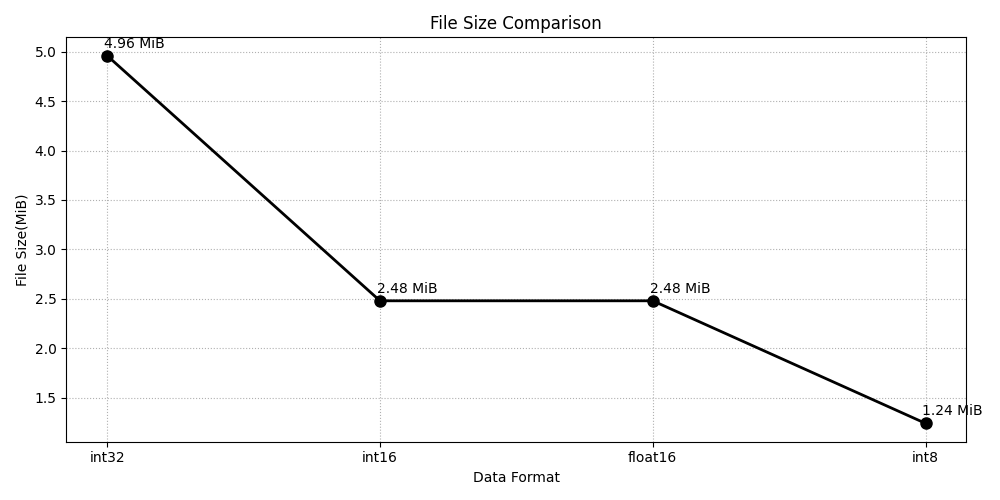
\includegraphics[height=0.4\textwidth]{assets/quantization/size_plot.png}
        \caption{File Size Comparision between Quantized Models}
        \label{fig:file-size-comparision}
    \end{figure}

    \begin{figure}[H]
        \centering
        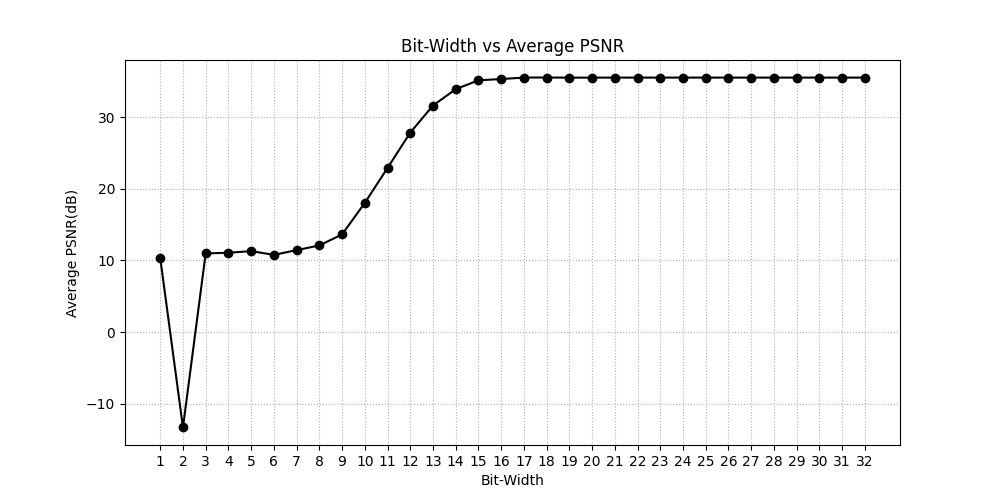
\includegraphics[height=0.4\textwidth]{assets/quantization/psnr.png}
        \caption{Average PSNR for Quantized Models}
        \label{fig:psnr-plot}
    \end{figure}

    \begin{figure}[H]
        \centering
        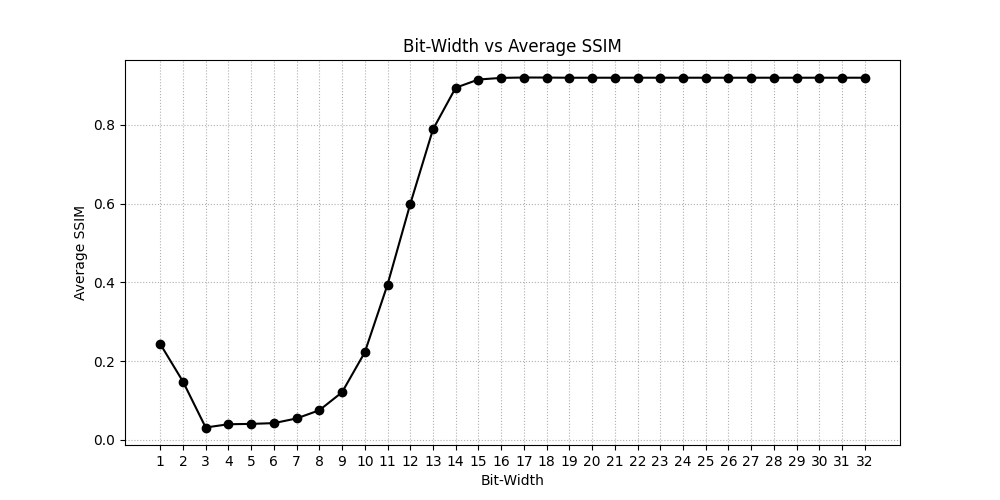
\includegraphics[height=0.4\textwidth]{assets/quantization/ssim.png}
        \caption{Average SSIM for Quantized Models}
        \label{fig:ssim-plot}
    \end{figure}

    \begin{figure}[H]
        \centering
        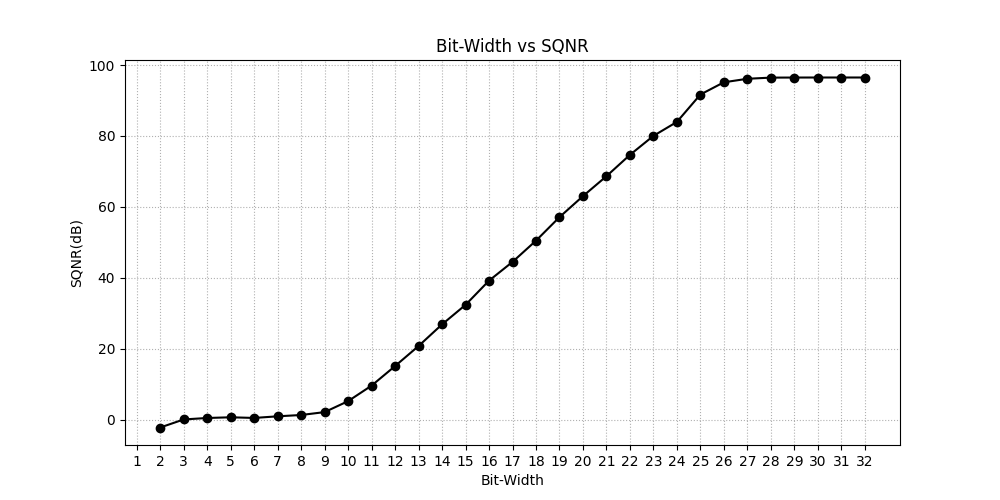
\includegraphics[height=0.4\textwidth]{assets/quantization/sqnr.png}
        \caption{SQNR for Quantized Models}
        \label{fig:sqnr-plot}
    \end{figure}

    The results, as observed from the graphs, show that quantizing the model to 16-bit integer results in reduction in file size. Moreover, both the \gls{ssim} and \gls{psnr} graphs indicate that reducing the bit-width initially affects these metrics, but from 16-bit onwards, the values stabilize, and further increase in bit-width has minimal impact on the model's accuracy. The \gls{sqnr} value for 16-bit quantization is also satisfactory. Given this balance between efficiency and performance, we chose to proceed with the 16-bit integer model for further experimentation and analysis. The results presented from this point onward are based on the 16-bit integer quantized model.

    \subsubsection{Visualization of Weight Quantization}
    The weight quantization process is depicted in \autoref{fig:quantization-sample-weights}, which consists of 3x3 grid of some sample weights. An example calculation is shown for the first weight in \autoref{app:quantization-manual-conversion}.
    \begin{enumerate}[label=\textbf{\roman*.}]
        \item \textbf{Original Weights:} The weights before quantization.
        \item \textbf{Quantized Weights:} The weights after quantization into 8-bit integers.
        \item \textbf{Integer Representation:} The representation of quantized weights in int8 format.
    \end{enumerate}

    \begin{figure}[H]
        \centering
        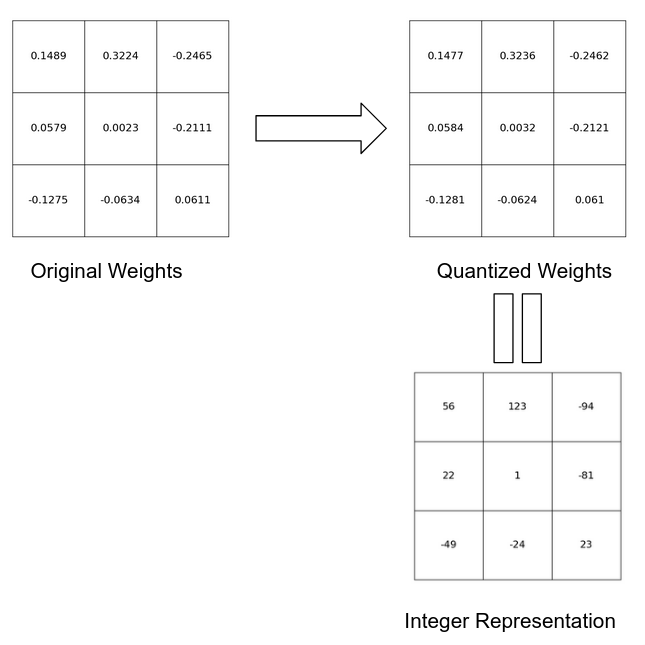
\includegraphics[width=0.8\linewidth]{assets/quantization/quantization_sample_weights.png}
        \caption{Quantization Sample Weights}
        \label{fig:quantization-sample-weights}
    \end{figure}

    \pagebreak

    \subsubsection{Histogram of Student Models}
    \autoref{fig:hist-student-vid1} and \autoref{fig:hist-student-vid3} show the histogram of weights and biases of the Student Model of Video 1 and Video 3.

    \begin{figure}[H]
        \centering
        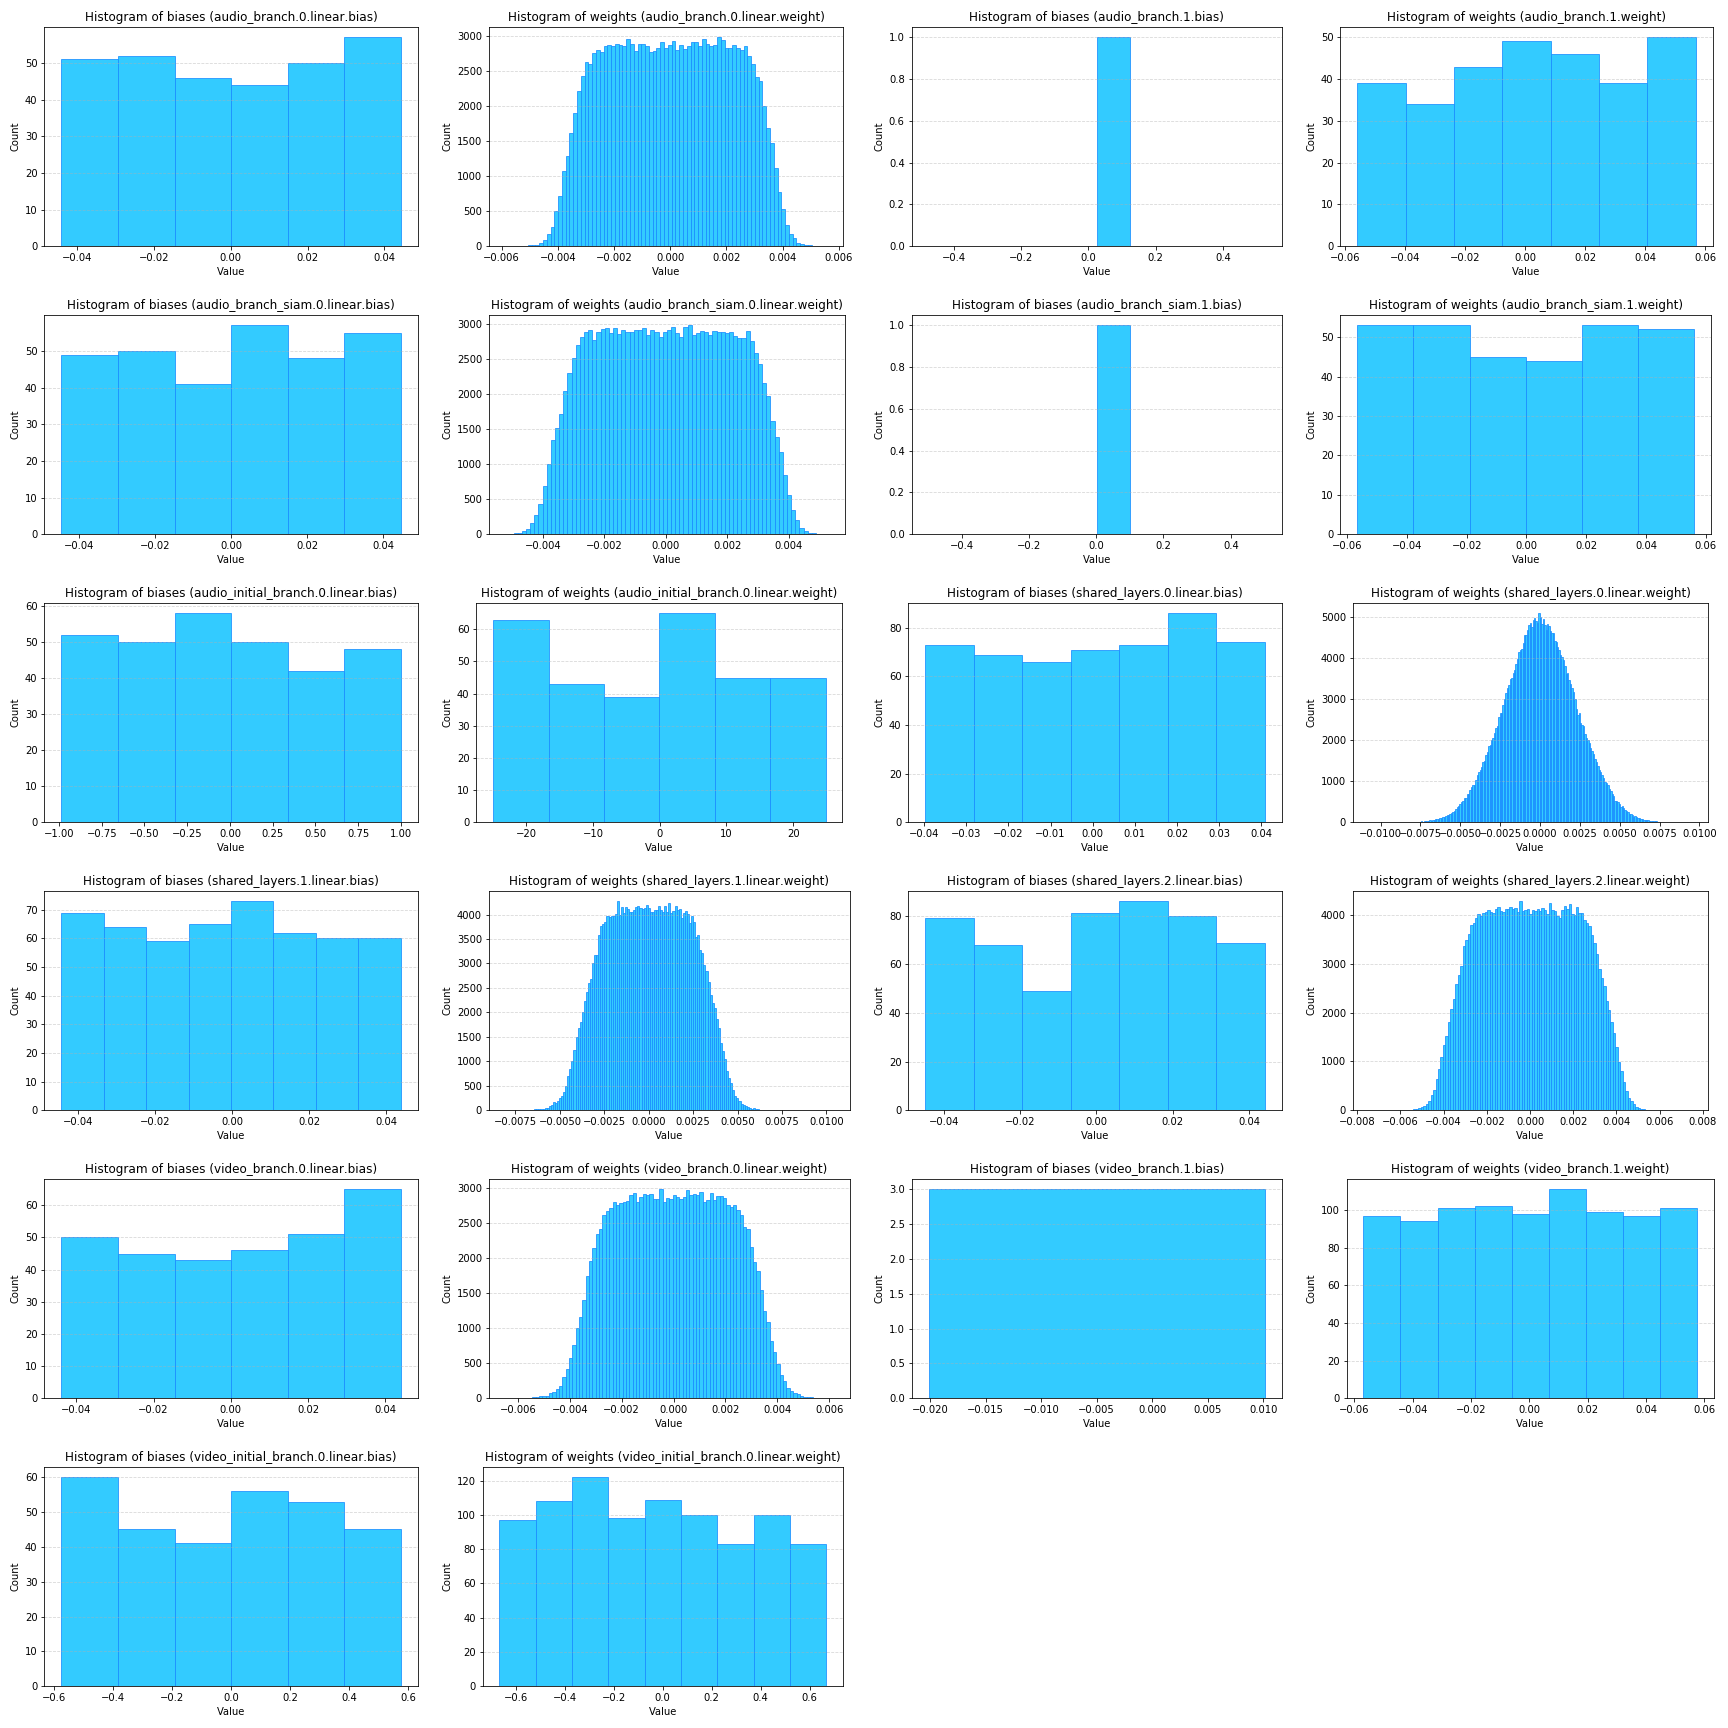
\includegraphics[width=\linewidth]{assets/quantization/histogram/histogram_vvsa_student.png}
        \caption{Histogram of Student Model:Video 1}
        \label{fig:hist-student-vid1}
    \end{figure}

    \begin{figure}[H]
        \centering
        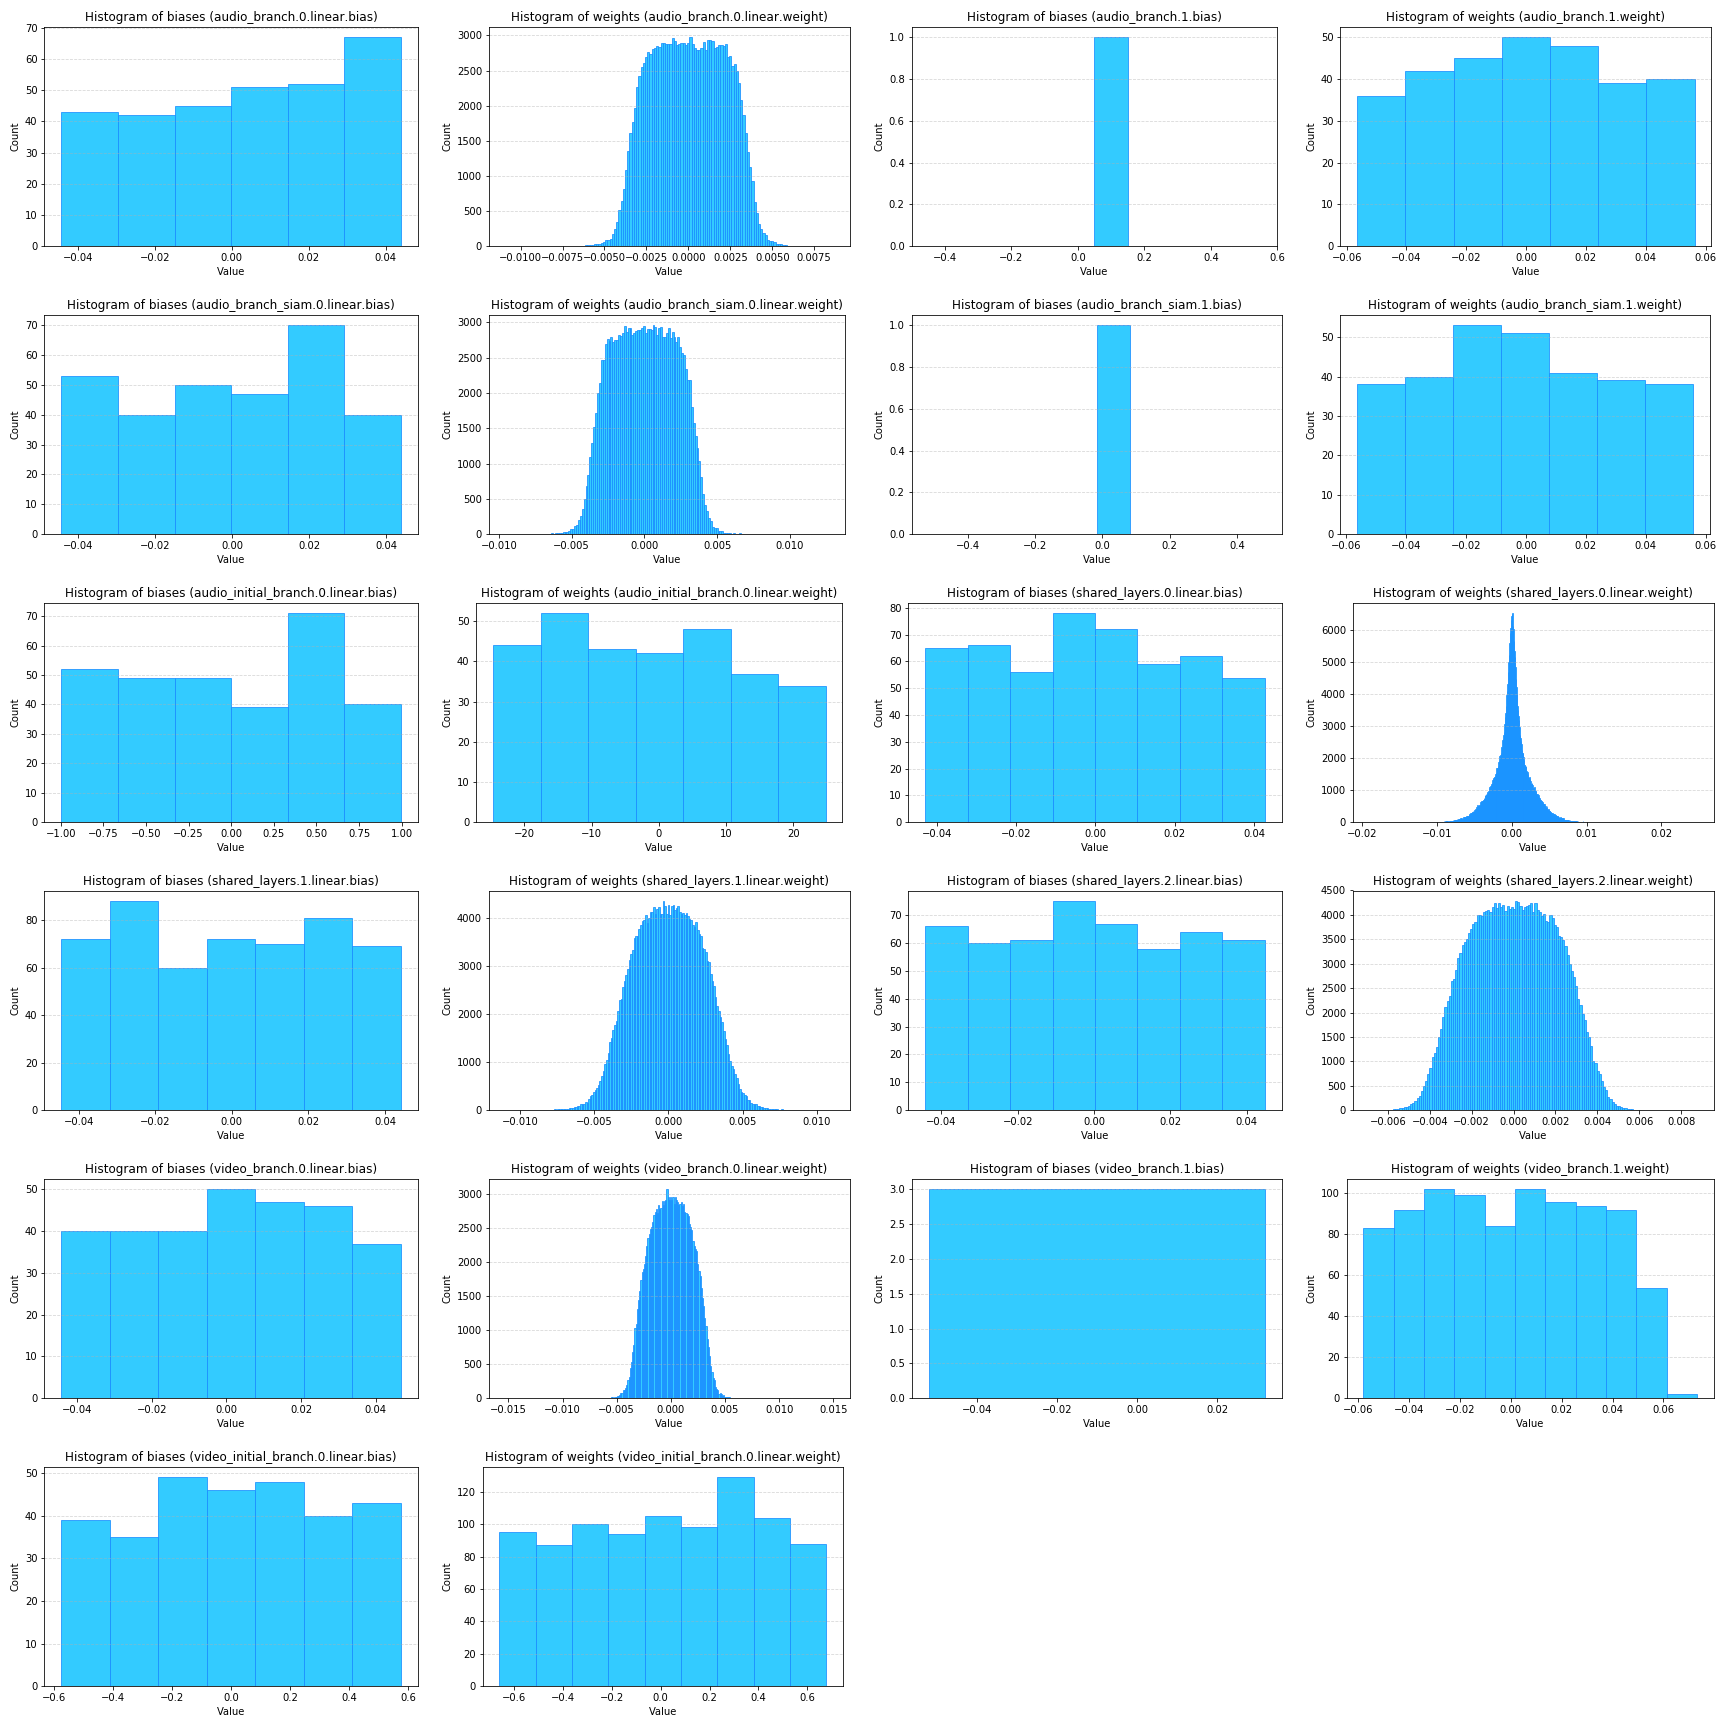
\includegraphics[width=\linewidth]{assets/quantization/histogram/histogram_rick_student.png}
        \caption{Histogram of Student Model:Video 3}
        \label{fig:hist-student-vid3}
    \end{figure}

    These histograms visualize the distributions of weights and biases for two student models across different layers and components, such as audio and video branches, shared layers, and initial layers. The distributions are diverse, with weights generally exhibiting Gaussian-like shapes centered around zero. Meanwhile, biases show more uniformly or slightlys skewed distribution.
    \pagebreak
